\section{Introduction}

After the discovery of Higgs boson~\cite{20121, 201230}, the examination of electroweak symmetry breaking (EWSB) becomes a main focus at the LHC.
In addition to measuring the properties of Higgs boson directly, the vector boson scattering (VBS) process is another key avenue to probe EWSB~\cite{Lee:1977yc, Chanowitz:1985hj, Szleper:2014xxa}.
As introduced in section~\ref{symbreaking}, in Standard Model (SM), the Higgs boson acts as ``moderator" to unitarize high-energy longitudinal VBS amplitudes at the ~\tev~ scale.
Therefore, studying high-energy behaviours of VBS is crucial to understand the mechanism of EWSB.

Since no VBS process was observed prior to the LHC era, LHC provides an exceptionable opportunity to study them due to its unprecedented high energy and luminosity.
At the LHC, the VBS process is typically studied through the measurements of electroweak (EW) production of two vector bosons radiated from quark-quark initial state, 
plus a pair of hadronic jets with high energy in the back and forward regions (denoted as EW-$VVjj$).
The quantum chromodynamics (QCD) production of $VVjj$ containing two QCD vertices at the lowest order (denoted as QCD-$VVjj$) is an irreducible background to the search of EW-$VVjj$ production.
The features of EW-$VVjj$ production including a large invariant mass of jet pair ($m_{jj}$) and a significant separation of rapidity between two jets ($\Delta y_{jj}$).
Figure~\ref{fig:vbszz_diagrams} presents some typical Feynman diagrams of EW- and QCD- $ZZjj$ processes.
\begin{figure}[!htbp]
\begin{center}
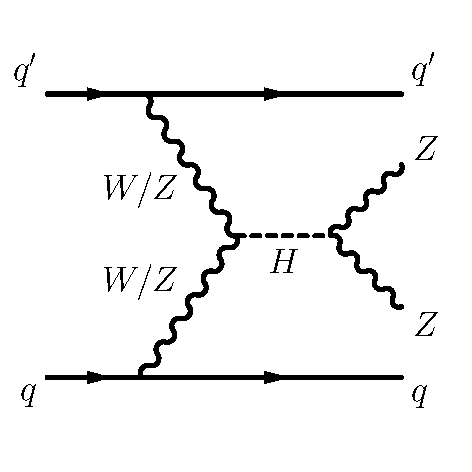
\includegraphics[width=0.22\textwidth]{figures/VBSZZ/diagram-EWZZjj-Schn-Higgs.pdf}
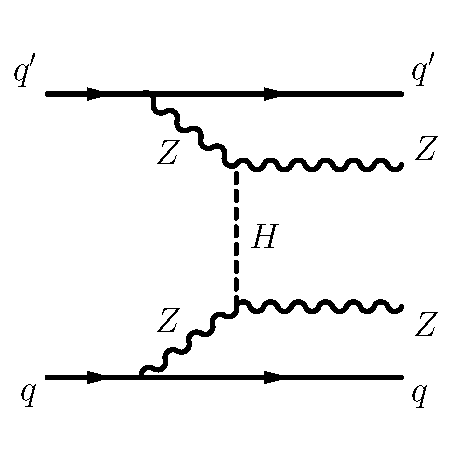
\includegraphics[width=0.22\textwidth]{figures/VBSZZ/diagram-EWZZjj-Tchn-Higgs.pdf}
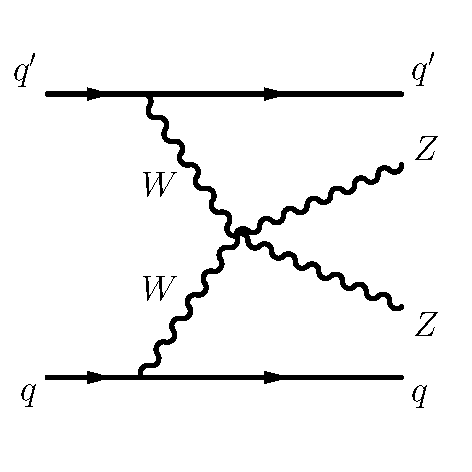
\includegraphics[width=0.22\textwidth]{figures/VBSZZ/diagram-EWZZjj-QGC.pdf}
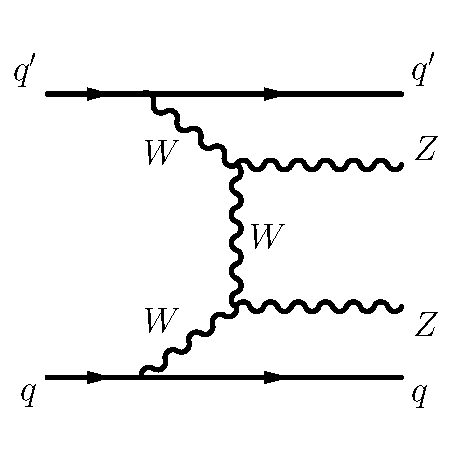
\includegraphics[width=0.22\textwidth]{figures/VBSZZ/diagram-EWZZjj-TGC.pdf}\\
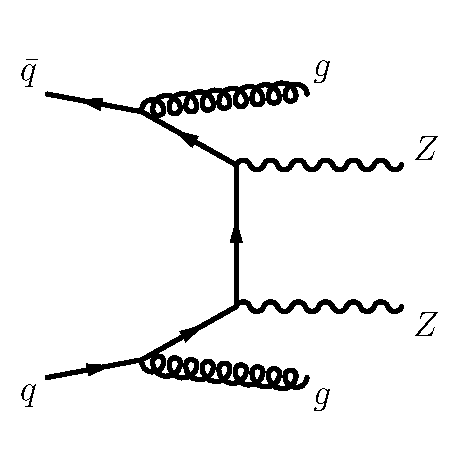
\includegraphics[width=0.22\textwidth]{figures/VBSZZ/diagram-QCDZZjj-qq.pdf}
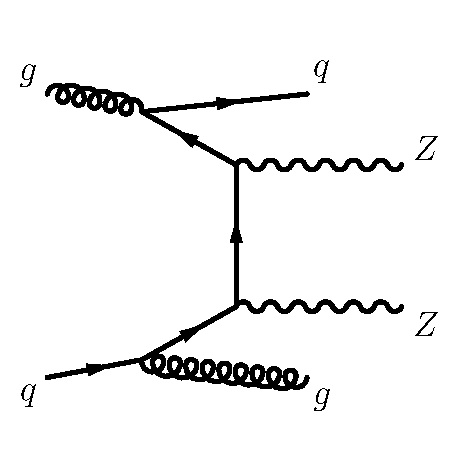
\includegraphics[width=0.22\textwidth]{figures/VBSZZ/diagram-QCDZZjj-qg.pdf}
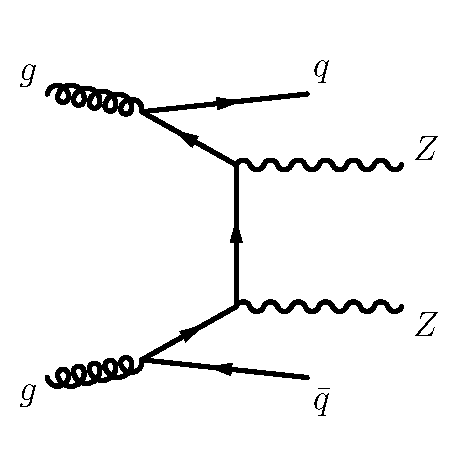
\includegraphics[width=0.22\textwidth]{figures/VBSZZ/diagram-QCDZZjj-gg.pdf}
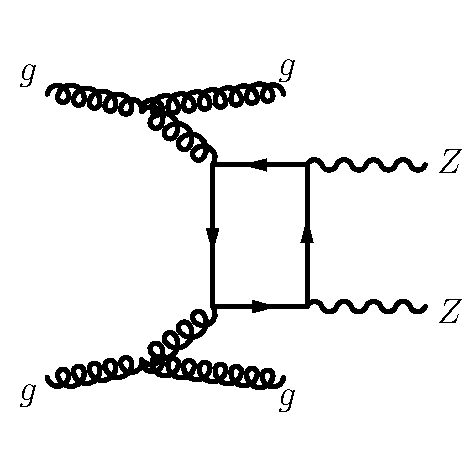
\includegraphics[width=0.22\textwidth]{figures/VBSZZ/diagram-QCDZZjj-box.pdf}\\
\end{center}
\caption{Typical diagrams for the production of $ZZjj$, including the relevant EW VBS diagrams (first row) and QCD diagrams (second row).}
\label{fig:vbszz_diagrams}
\end{figure}

The first evidence of the EW-$VVjj$ process was seen in same-sign $WW$ channel (EW-$W^{\pm}W^{\pm}jj$) by ATLAS collaboration with 20.3~\ifb~8~\tev~data~\cite{PhysRevLett.113.141803},
in which a 3.6$\sigma$ excess was observed in data over the background-only prediction.
In the LHC run-2, the observation (with > 5 $\sigma$ statistical significance) of EW-$W^{\pm}W^{\pm}jj$ process has been reported in both ATLAS and CMS collaboration with 36~\ifb~13~\tev~data\cite{PhysRevLett.123.161801, Sirunyan:2017ret}.
In $WZ$ channel (EW-$WZjj$), an observation with 5.3 $\sigma$ excess was also reported by the ATLAS collaboration recently~\cite{2019469}.
As for the EW-$ZZjj$ production, it was searched by CMS using 35.9~\ifb~13~\tev~data but no evidence was found\cite{2017682}.
The EW production in $ZZ$ final state (EW-$ZZjj$) is typically rare, whose fiducial cross section has an order of \textit{O}(0.1)~\ifb in the final state where both $Z$ bosons decay leptonically.
But in the meantime, $ZZ \rightarrow \llll$ process offers an extremely clean channel than all the others. So with more data collected in the LHC, the observation of EW-$ZZjj$ becomes possible.

This section presents the first observation of EW-$ZZjj$ production decaying to four charged leptons with two jets (\lllljj) by ATLAS collaboration using the complete set of the LHC run-2 data with 139~\ifb luminosity~\cite{Aad:2020zbq,Zhu:2714092}.
It is a new milestone in the study of EWSB at the LHC, and completes the last missing part of observation of weak boson scattering for massive bosons.
In the meatime, the measurement of fiducial cross-sections for SM $ZZ$ production including both EW and QCD processes is also reported.
The $ZZjj$ production involving intermediate $\tau$-leptons from $Z$ decays is considered as signal but has a negligible contribution to the selected events.
Reducible backgrounds give minor contributions in the \lllljj channel are also studied.
To further separate the EW signal and the QCD background, multivariate discriminant (MD) is trained using event kinematic information from simulated samples. 
The MD distribution is then used as discriminant in statistical fit to evaluate the signal strength of EW process.
